\documentclass[brazil,a4paper,12pt]{article}

\usepackage{amsmath}
\usepackage{fullpage}
\usepackage{fancyvrb}
\usepackage[brazil]{babel}
\usepackage[utf8]{inputenc}
\usepackage{graphicx}
\usepackage{booktabs}

\DeclareMathOperator*{\argmax}{arg\,max}

\begin{document}

\begin{center}
\LARGE
\textbf{Mineração de Dados}\\
\textbf{TP4: Reconhecimento de Faces}\\
\end{center}
\begin{center}
\textbf{Aluno: Flavio Vinicius Diniz de Figueiredo}
\end{center}

\section{Descrição}

O objetivo do TP foi de realizar uma proposta de um sistema de mineração de
dados para o reconhecimento de faces de funcionários de uma empresa. Foi
disponibilizado 10 fotos para cada um de 15 funcionários, um total de 150 fotos, 
da empresa para realizar a tarde. Abaixo detalhamos melhor o problema 
especificado no TP.

\begin{description}

\item [Técnica de Classificação] Foi requisitado de cada aluno a implementação de
uma técnica de mineração de dados para o problema de reconhecimento de faces.

\item [Sistema de Reconhecimento] Após a implementação de técnica, foi
requisitado uma proposta de sistema que fizesse uso da mesma para ser
implementado na empresa. Para a avaliação do sistema, um subconjunto de fotos
de um funcionário deve ser usado como teste do sistema. 

\end{description}

\section{Classificação de Faces}

O conjunto de dados originais era composto de 150 fotos, sendo 10 fotos para
cada um de 15 funcionários da empresa. As fotos de casa funcionário diferem
no uso de acessórios como óculos e expressões faciais. Cada foto tem o formato
BMP sendo composto de uma matriz de 100x100 pixels em grey-scale 
(intensidade no intervalo $[0, 256)$).

\subsection{Pre-Processamento}

Inicialmente transformados cada imagem em um vetor de 10000 elementos. Isto é
feito concatenando cada umas das 100 linhas de 100 elementos da imagem original
em um vetor único. Abaixo mostramos um exemplo do processo:

A matriz:

\[
 A_{m,n} =
 \begin{pmatrix}
  a_{1,1} & a_{1,2} & \cdots & a_{1,n} \\
  a_{2,1} & a_{2,2} & \cdots & a_{2,n} \\
  \vdots  & \vdots  & \ddots & \vdots  \\
  a_{m,1} & a_{m,2} & \cdots & a_{m,n}
 \end{pmatrix}
\]

\noindent se torna:

\[
\mathbf{a}_{m \times n} =
<a_{1,1}, a_{1,2} \cdots a_{1,n} \cdots a_{m,1}, a_{m,2} \cdots a_{m,n}>
\]
.

\noindent Com isto, cada imagem tem 10000 atributos que equivale a 
i tensidade de cada pixel. Após a transformação das imagens em vetores,
construímos um outro vetor de labels das imagens originais. Este é
usado para realizar o treino e teste da classificação.

No contexto de reconhecimento de faces, o uso de vetores de alta 
dimensão como os gerados geralmente leva a uma baixa eficácia
~\cite{turk1991eigenfaces}. O motivo disto é falha é que a técnica
de aprendizado pode considerar variações de expressão/acessórios/luz como
sendo outras pessoas, pois uma grande quantidade de pixels vão ser
diferentes entre as duas imagens. Para resolver este problema, uma técnica
comum é representar cada imagem em um espaço de menor dimensão. Aplicamos
o uso de {\it Principal Component Analysis (PCA)} para fazer esta redução.
É conhecido a eficácia de PCA neste contexto, iremos detalhar em mais detalhes
como PCA foi usado neste tarefa abaixo~\cite{turk1991eigenfaces}.

\begin{figure}
\centering
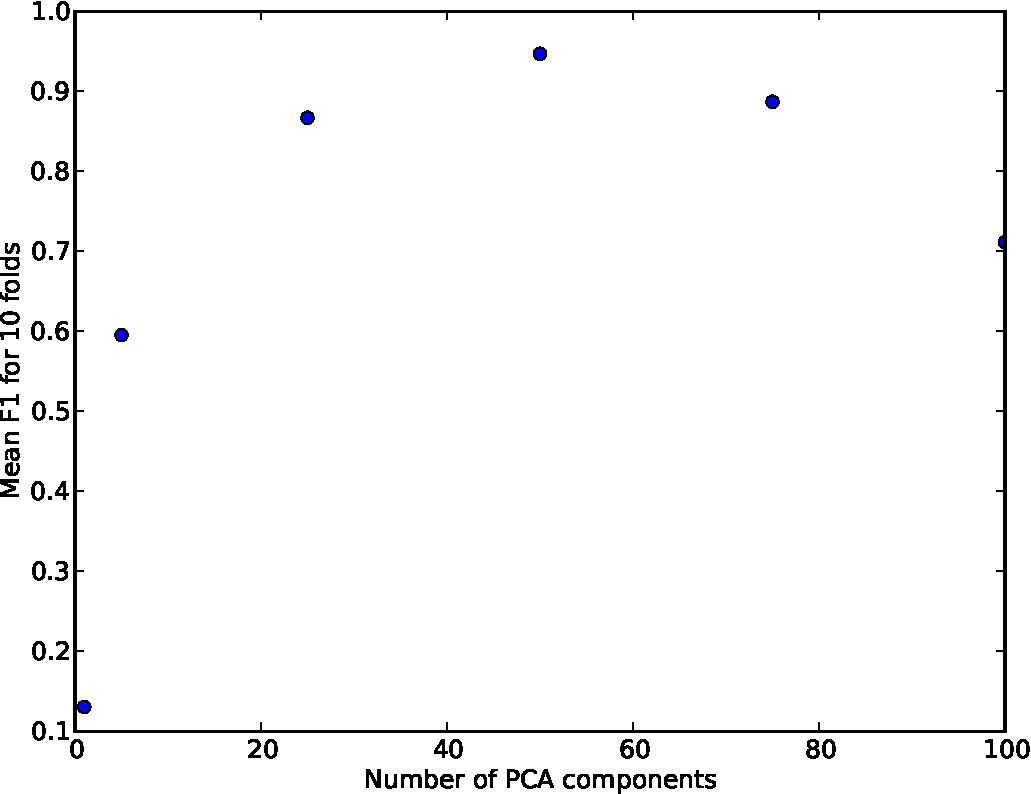
\includegraphics[scale=0.6]{pca-crop.pdf}
\caption{Eficácia do uso de PCA}
\label{fig:groups}
\end{figure}

Após a transformação de imagens em vetores, precisamos escolher a dimensão
do novo espaço que queremos gerar com o uso de PCA. Para isto, realizamos
os seguintes passos: (1) buscamos o melhor número de dimensões considerando
os valores ${2, 5, 25, 50, 75, 100}$; (2) para cada um deste valores, 
transformamos os dados usando PCA; (3) nos dados transformados, buscamos
o melhor classificador SVM variando o custo e o gamma com um kernel $rbf$
~\cite{meira};
(4) escolhemos o melhor modelo de SVM para cada dimensão, avaliado com 
a métrica Micro-F1~\cite{meira}; (5) escolhemos a melhor 
quantidade de dimensões,
aquela que maximiza o melhor Micro-F1 para cada dimensão. 
Na página seguinte mostramos o pseudo-código que sumariza a análise.

Para cada valor de nova dimensionalidade considerado, plotamos na 
Figura~\ref{fig:groups} a média do valor de Micro-F1 para para cada
uma análise de {\it 10-fold cross validation}~\footnote{Geramos folds de de forma
que a proporção de elementos de cada classe fosse mantida no treino e teste. 
Neste tipo de análise $90\%$ dos dados são treino e $10\%$ são testes. Em geral,
no entre 1 e 2 fotos de cada classe era usada para teste.} 
nos dados transformados usando PCA. 
Pela figura, podemos ver que o melhor valor para números de dimensões é 50.

\begin{verbatim}
using: X as data matrix, y as labels vector

new_dims = [2, 5, 25, 50, 75, 100]
pca_models = []

for new_dim in new_dims
    
    new_data = pca(X, new_dim)
    cv = cross_val(X, y, 10)

    mean_f1_scores = []
    models = []

    for cost in [1, 5, 10, 50, 100]
        for gamma in [0.0001, 0.0005, 0.001, 0.005, 0.01, 0.1]

            f1_scores = []
            for train, test in cv:

                X_train = X[train]
                y_train = y[train]
        
                X_test = X[test]
                y_test = y[test]
        
                model = svm_train('rbf', X_train, y_train, cost, gamma)
                y_predict = svm_predict(model, X_train)
                f1_score = f1(y_test, y_predict)
                f1_scores.append(f1_score)
            done

            models.append( (cost, gamma) )
            mean_f1_scores.append(mean(f1_scores))
        done
    done
    i = find_max(mean_f1_scores)

    pca_models.append(models[i])
done

i = find_max(pca_f1)
return pca_new_dim[i], pca_models[i]

\end{verbatim}

\section{Eficácia do Algoritmo}


Após fazer uso de PCA para reduzir o espaço de 10000 dimensões para 50 
dimensões, assim como escolher o melhor modelo de SVM ($C=0$ e $\gamma=0.001$);
rodamos novamente uma análise de {\it 10-fold cross validation} para a mensurar
a eficácia da classificação.

Para cada um dos 10 folds, realizamos uma análise de métricas comum de classificação,
sendo estas a Precisão, Revocação, Micro-F1 e Suporte~\cite{meira}. Abaixo mostramos
um exemplo de resultados para um dos nossos folds:

\begin{verbatim}
Fold 0 - report
             precision    recall  f1-score   support

          1       1.00      1.00      1.00         1
          2       1.00      1.00      1.00         1
          3       1.00      1.00      1.00         1
          4       0.00      0.00      0.00         1
          5       1.00      1.00      1.00         1
          6       1.00      1.00      1.00         1
          7       1.00      1.00      1.00         1
          8       1.00      1.00      1.00         1
          9       1.00      1.00      1.00         1
         10       1.00      1.00      1.00         1
         11       1.00      1.00      1.00         1
         12       1.00      1.00      1.00         1
         13       1.00      1.00      1.00         1
         14       1.00      1.00      1.00         1
         15       0.50      1.00      0.67         1

avg / total       0.90      0.93      0.91        15

Fold 0 - confusion matrix
[[1 0 0 0 0 0 0 0 0 0 0 0 0 0 0]
 [0 1 0 0 0 0 0 0 0 0 0 0 0 0 0]
 [0 0 1 0 0 0 0 0 0 0 0 0 0 0 0]
 [0 0 0 0 0 0 0 0 0 0 0 0 0 0 1]
 [0 0 0 0 1 0 0 0 0 0 0 0 0 0 0]
 [0 0 0 0 0 1 0 0 0 0 0 0 0 0 0]
 [0 0 0 0 0 0 1 0 0 0 0 0 0 0 0]
 [0 0 0 0 0 0 0 1 0 0 0 0 0 0 0]
 [0 0 0 0 0 0 0 0 1 0 0 0 0 0 0]
 [0 0 0 0 0 0 0 0 0 1 0 0 0 0 0]
 [0 0 0 0 0 0 0 0 0 0 1 0 0 0 0]
 [0 0 0 0 0 0 0 0 0 0 0 1 0 0 0]
 [0 0 0 0 0 0 0 0 0 0 0 0 1 0 0]
 [0 0 0 0 0 0 0 0 0 0 0 0 0 1 0]
 [0 0 0 0 0 0 0 0 0 0 0 0 0 0 1]]
\end{verbatim}

Para sumarizar para os vários folds, mensuramos a média do Micro-F1 encontrado,
este valor foi de $0.946667$, mostrando a eficácia da nossa técnica. No arquivo
de resultados entregue junto com o TP mostrados em detalhes tais resultados.

\section{Sistema de Reconhecimento}

\begin{figure}
\centering
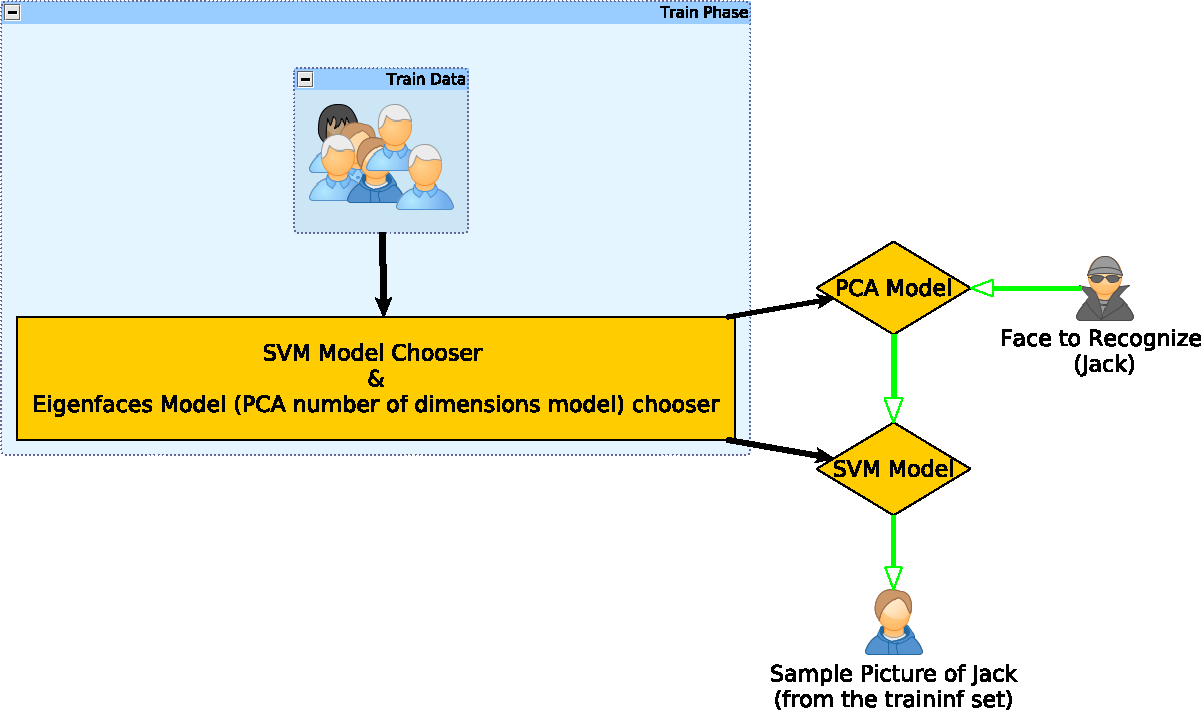
\includegraphics[scale=0.6]{sys-crop.pdf}
\caption{Esboço de Sistema}
\label{fig:sys}
\end{figure}

\begin{figure}
\centering
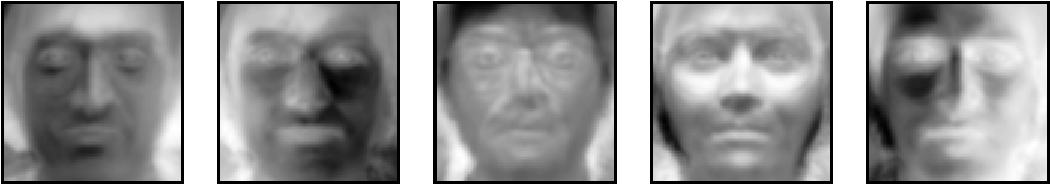
\includegraphics[scale=0.6]{eig-crop.pdf}
\caption{Eigenfaces}
\label{fig:eig}
\end{figure}

Por fim, o TP requisitou um esboço de sistema de detecção de faces para uso na
empresa. Na Figura~\ref{fig:sys} apresentamos um esboço do sistema. Periodicamente,
toda noite por exemplo, a empresa pode treinar um novo modelo de PCA e um novo modelo
de SVM usando um algoritmo como o descrito anteriormente. Com tais modelos, é possível
reduzir a quantidade de dimensões de cada foto de funcionário para ser identificado,
após isto é possível extrair do sistemas um conjunto de fotos passadas (que foram
usadas no treino) e / ou o nome do funcionário para a identificação. Na Figura~\ref{fig:eig} 
exemplificamos o modelo de PCA treinado demonstrando alguma ``eigenfaces''.

Para avaliar um esboço de tal sistema, implementamos o mesmo escondendo 3 fotos de um usuário
na fase de teste. Verificamos que o sistema sempre detecta o usuário corretamente, obtendo
um valor máximo de F1 ($1$) sempre. Repetimos isto para todas as combinações possíveis de 3
fotos deste mesmo usuário e sempre obtivemos o resultado ótimo.

\bibliographystyle{plain}
\bibliography{bibs}

\end{document}
